\begin{enumerate}\setcounter{enumi}{1}\bfseries
    \item \textbf{Apresente uma notícia recente de um problema de Ética em IA.}
\end{enumerate}

O site de notícias \textit{The Verge} publicou o artigo \textit{Anyone can use this AI generator - that's the risk} \cite{verge_ai_generator}. A notícia discute o avanço da inteligência artificial na área de programas de texto-para-imagens. Esses programas abriram a possibilidade para que pessoas sem habilidades artísticas pudessem, com prompts de texto, gerar imagens através da inteligência artificial, que utiliza de uma vasta base de imagens para gerar o pedido.

A inteligência artificial está longe de ser perfeita. Ela possui problemas para gerar mãos, ocasionalmente existem deformidades nas pessoas, entre outras falhas. Entretanto, essas falhas não são incômodas para quem está empolgado com a tecnologia, que pode gerar qualquer imagem que você pode imaginar.

% Código para centralizar uma figura e posicioná-la "exatamente" no texto
% O opção 'h' posiciona a imagem
% \centering dentro do ambiente figure centraliza
\begin{figure}[h]
\centering
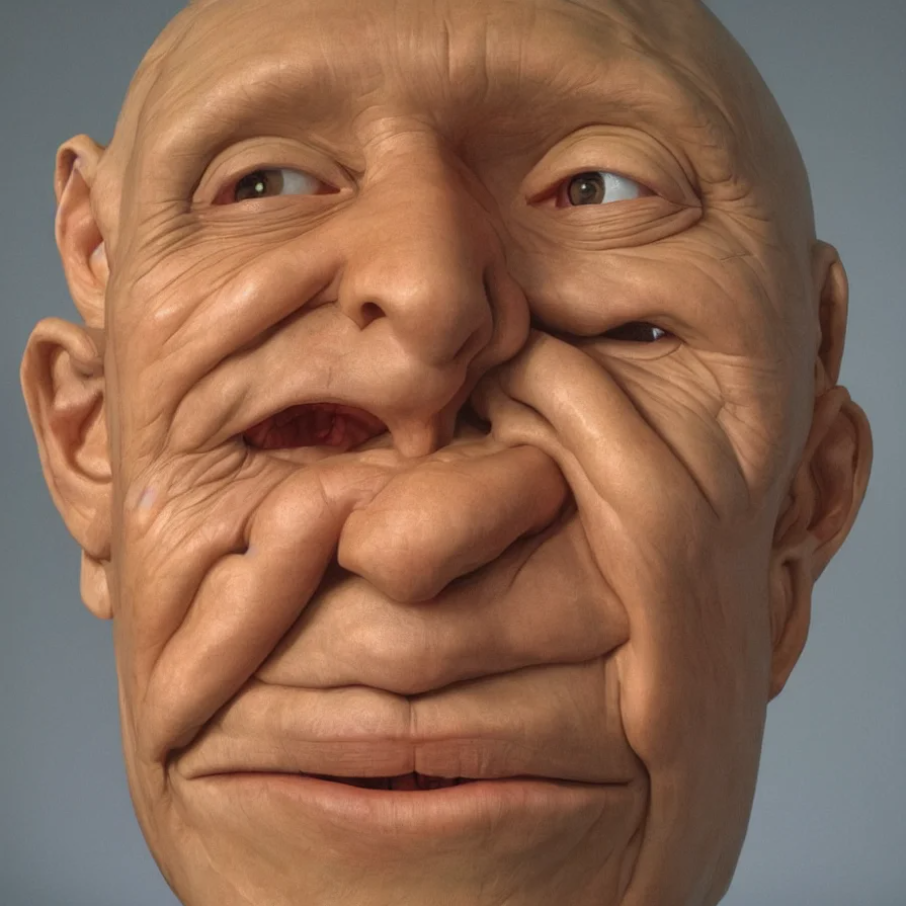
\includegraphics[scale=0.15]{face_deformada.png}
\caption{Imagem gerada por um prompt pedindo uma escultura hiperrealista de uma face humana. Encontrada no \href{https://lexica.art/prompt/10023e09-97d2-4ba3-8e01-4ee149a42c6f}{Lexica}.}
\end{figure}


A empresa OpenAI possui o gerador de imagens \textit{DALL-E}, que possui uma quantidade finita de geração de imagens gratuitas por mês. Após esta quantidade se esgotar é necessário pagar por prompts para gerar novas imagens, criando uma pequena barreira para aqueles que querem gerar imagens. O Google possui um gerador de imagens chamado \textit{Imagen}, mas este não está aberto ao público.

